\Testart{Skript}
\Klasse{10}
\Fach{Informatik}
\Titel{Datenbanken (Teil 1)}

\renewcommand{\Content}{
    
    \mysession{Stunde 1+2}{
        \Hefteintrag{1.8}{Wdh: Klassen und Objekte}{
    \emphColA{\LoesungLuecke{Objekte}{5cm}} repräsentieren \emphColA{Gegenstände} in einem Computerprogramm. \emphColB{\LoesungLuecke{Klassen}{5cm}} sind der \emphColB{Bauplan}, der festlegt, welche \emphColC{Eigenschaften} (\emphColC{\LoesungLuecke{Attribute}{5cm}}) und \emphColor{red}{Fähigkeiten} (\emphColor{red}{\LoesungLuecke{Methoden}{5cm}}) einer bestimmten Objektart gespeichert werden sollen. Man stellt sie dar mit:

    %\vspace{0.1cm}
    \begin{minipage}[t]{0.32\textwidth}
        \centering
        \Large \emphColB{Klassenkarte}

        \vspace{0.1cm}
        \LoesungKaroTikz{
            \begin{class}[text width=\textwidth]{Person}{0,0}
                \attribute{String hobby}
                \attribute{int alter}
                \attribute{boolean hatHaustier}
                \attribute{String peinlichesErlebnis }
                \operation{void atmen()}
            \end{class}
        }{15}
        \Loesung{spitze Ecken}
    \end{minipage}
    \hfill
    \begin{minipage}[t]{0.3\textwidth}
        \centering
        \Loesung{
            \vspace{0.1cm}
            
            {\flushright
            $\leftarrow$ Klassenname}

            \vspace{-5pt}
            {\flushleft
            Objektname~:~Klassenname $\rightarrow$}

            \vspace{1cm}
            Attribute

            \vspace{2cm}
            {\flushright
            $\leftarrow$ Methoden}
        }
    \end{minipage}
    \hfill
    \begin{minipage}[t]{0.32\textwidth}
        \centering
        \Large \emphColA{Objektkarte}

        \vspace{0.1cm}
        \LoesungKaroTikz{
            \begin{object}[text width=\textwidth]{p1 : Person}{0,0}
                \attribute{hobby = "Klettern"}
                \attribute{alter = 23}
                \attribute{hatHaustier = false}
                \attribute{peinlichesErlebnis = "..."}
            \end{object}
        }{15}
        \Loesung{runde Ecken}    
    \end{minipage}
    
    \setstretch{1.0}
    \hinweis{Generell kann man Objektkarten mit oder ohne Methoden zeichnen, solange man es insgesamt einheitlich macht. Wir zeichnen sie daher immer \underline{ohne Methoden}.}
}

        \Aufgabe{Objektkarten Memory}{
    \doppelseite{0.4}{0.45}{t}{
        \begin{itemize}
            \item Erstelle auf einem Blatt eine Objektkarte der Klasse Person zu dir selbst. $\rightarrow$ \emphColA{3x falten}
            \item Gib deine Objektkarte bei der Lehrkraft ab. $\rightarrow$ Objektkarten werden gemischt.
            \item Ziehe eine Objektkarte und versuche, das zugehörige Objekt zu finden.
            \begin{itemize}
                \item Frage deine:n Gegenüber dafür, ob die Attributwerte auf deiner gezogenen Karte auf sie/ihn zutreffen.
                \item Ihr dürft euch nicht gegenseitig die Objektkarten zeigen!
                \item Wer gefunden wurde, gibt seine aktuelle Objektkarte weiter und setzt sich.
                \item Der/Die Finder:in sammelt alle gefundenen Objekte.
            \end{itemize}
        \end{itemize}
    }{
        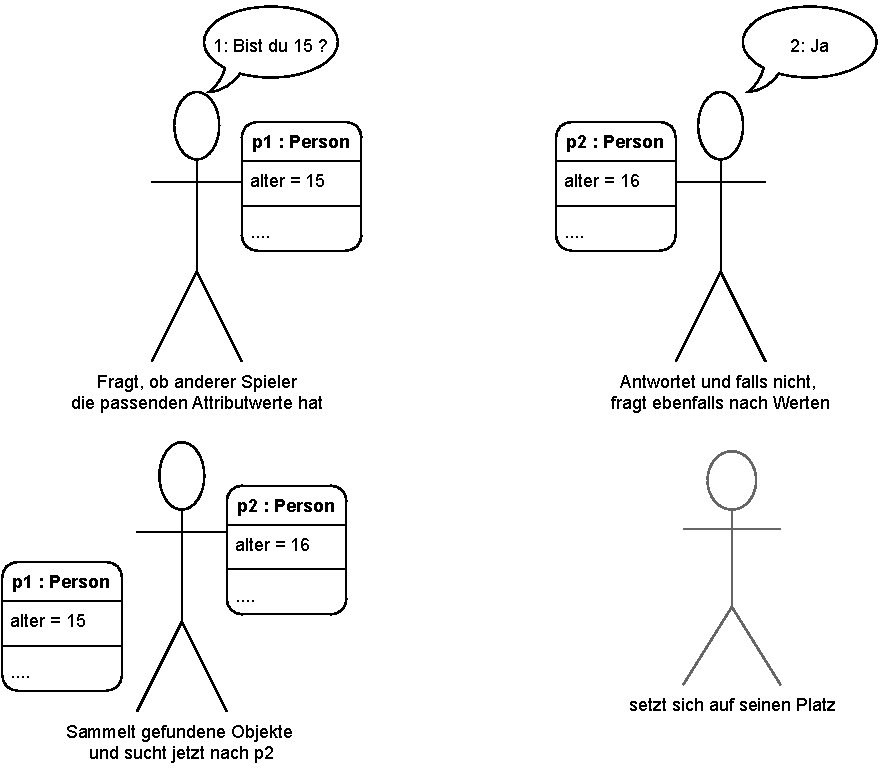
\includegraphics[width=\linewidth]{_Aufgaben/img/A00_Diagramm.pdf} 
    }
}


    }
    \mysession{Stunde 3+4}{
        \Aufgabe[20]{Wdh: Von der Klasse zur Tabelle}{
    \begin{itemize}
        \item Zeichnet zu zweit eine Tabelle, in der man alle Objekte der Klasse Person sammeln kann.
        \item Tragt eure beiden Objekte (vom Objektkarten-Memory) in die Tabelle ein.
        \item Ordnet die folgenden Begriffe den Teilen der Tabelle zu.
            \\Achtung: Nicht alle Begriffe passen und manches hat mehrere Begriffe!
            \\
        \emphColB{Datensatz~~~ Tabelle~~~ Zelle~~~ Klasse~~~ Objekt~~~ Parameter~~~ Attribut~~~ Spalte~~~ Feld~~~ Methode~~~ Board~~~ Zeile~~~ Datentyp~~~ Attributwert}
    \end{itemize}
    \LoesungKaro{
        Lösung:
        
        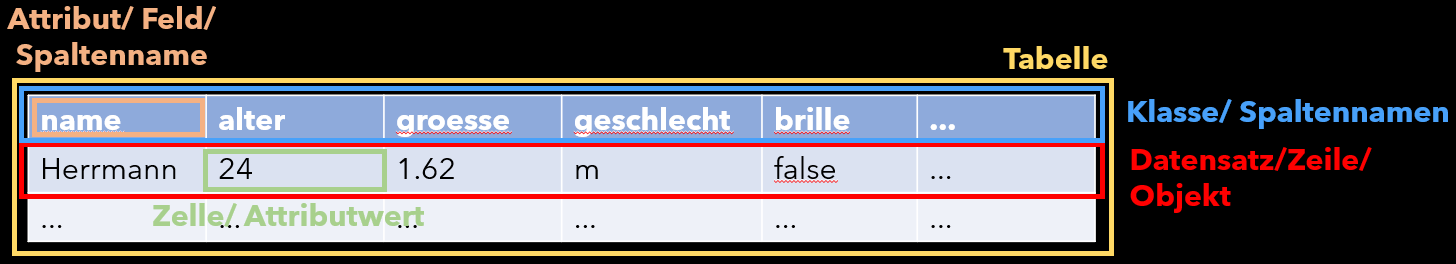
\includegraphics[width=\textwidth]{_Aufgaben/img/A01_Lsg.png}

        Nicht verwendete Begriffe: Parameter, Methode, Board, Datentyp

        \footnotesize
        Feld: Wird oft synonym zu Attribut verwendet, v.a. in Programmen wie LibreOffice Base oder MS Access.
    }{17}
}


        \Hefteintrag{1.5}{Wdh: Aufbau von (relationalen) Datenbanken}{

    Datenbanken speichern Datensätze in \emphColA{\LoesungLuecke{Tabellen}{5cm}}. Die \emphColB{\LoesungLuecke{Spaltenüberschriften}{7cm}} repräsentieren die \emphColB{Attribute} (Synonym: Feld) und bilden zusammen eine \emphColor{yellow}{Klasse}. Die \emphColC{\LoesungLuecke{Datensätze}{5cm} (=Zeilen)} entsprechen \emphColC{Objekten} und in den Spalten stehen die Attributwerte.
    Jede Tabelle hat einen \emphColor{red}{\LoesungLuecke{Primärschlüssel}{6cm} (oft auch „ID“)}, der Datensätze eindeutig identifiziert. Oft werden die Datensätze hiermit einfach durchnummeriert. Im Tabellenschema wird er unterstrichen und im Klassendiagramm immer als erstes Attribut aufgelistet.
    
    Der Aufbau einer Tabelle kann mit  \emphColA{\LoesungLuecke{Klassenkarte}{5cm}} oder \emphColA{\LoesungLuecke{Tabellenschema}{5cm}} dargestellt werden. Dessen Aufbau ist:

    {
        \fontfamily{pcr}\selectfont
        \textbf{TABELLENNAME(\underline{Datentyp Primärschlüssel} , Datentyp Spalte1, Datentyp Spalte2, …)}
    }

        Zum Beispiel:

        \LoesungLine{Person(\underline{int id}, String name, int alter, …)}{1}
    
}

        \Hefteintrag{1}{SQL Spickzettel}{
    \AttachVlg{\faFilePdfO}{_Hefteintraege/img/SQL-Spickzettel_2on1.pdf}

    \ifbeamer\else\vspace{12pt}\fi
    Folgender SQL-Spickzettel enthält alle SQL-Grundlagen der 9. Klasse. Ihr dürft (sollt!) ihn bei allen SQL-Aufgaben benutzen. Über das Vorlagensymbol~~~\faFilePdfO~~~ oben könnt ihr den Spickzettel als eigenes PDF öffnen.
    
    \hinweis{Übrigens: \emphColA{SQL} ist die Abkürzung für \emphColA{S}tructured \emphColA{Q}uery \emphColA{L}anguage, was auf Deutsch etwa Strukturierte Abfrage Sprache heißt.}
    \begin{tcolorbox}[
        boxrule=0pt,        % Kein Rand um die Box
        enhanced,           % Erweiterte Optionen aktivieren
        colback=white,      % Hintergrundfarbe der Box auf Weiß setzen
        frame hidden,       % Rahmen ausblenden
        boxsep=-10mm
    ]
        \centering
        \ifbeamer
            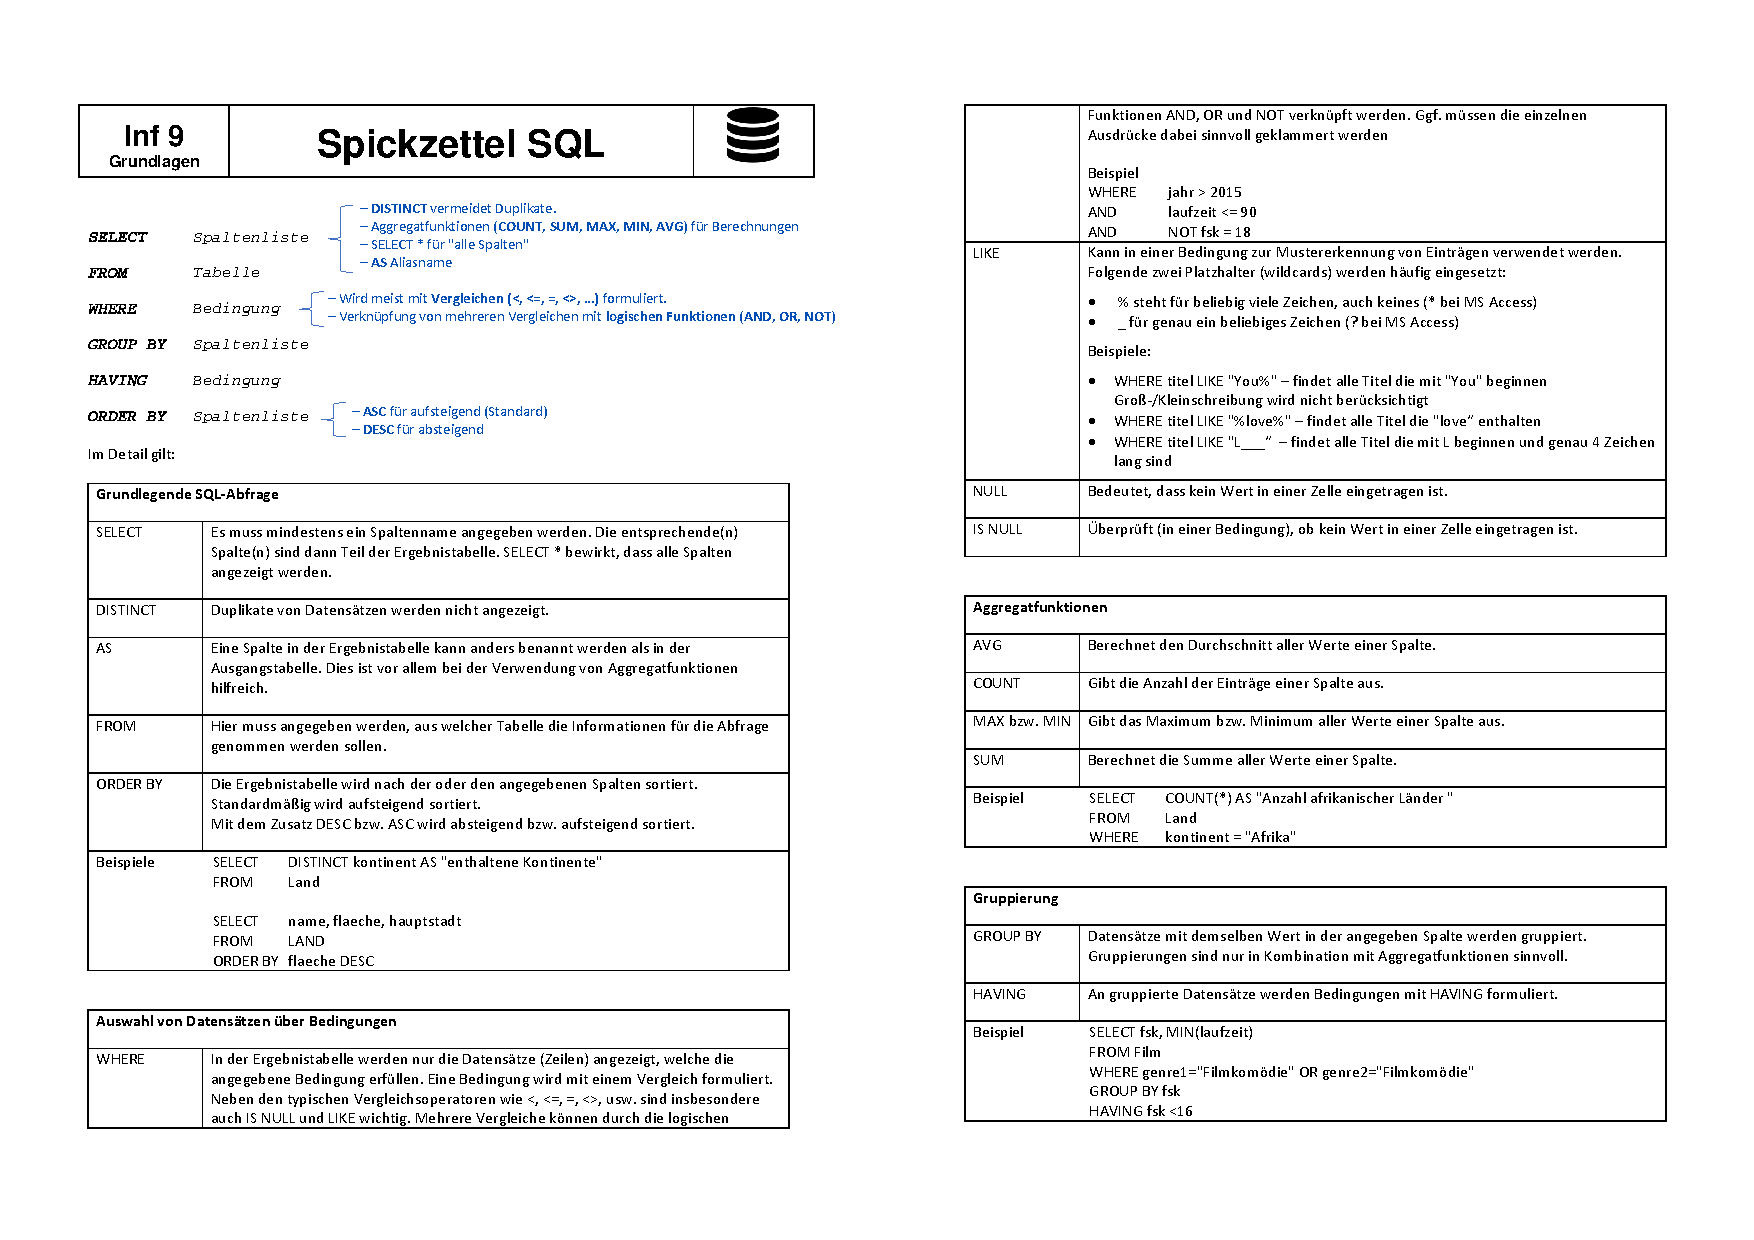
\includegraphics[width=0.68\textwidth]{_Hefteintraege/img/SQL-Spickzettel_2on1.pdf}
        \else
            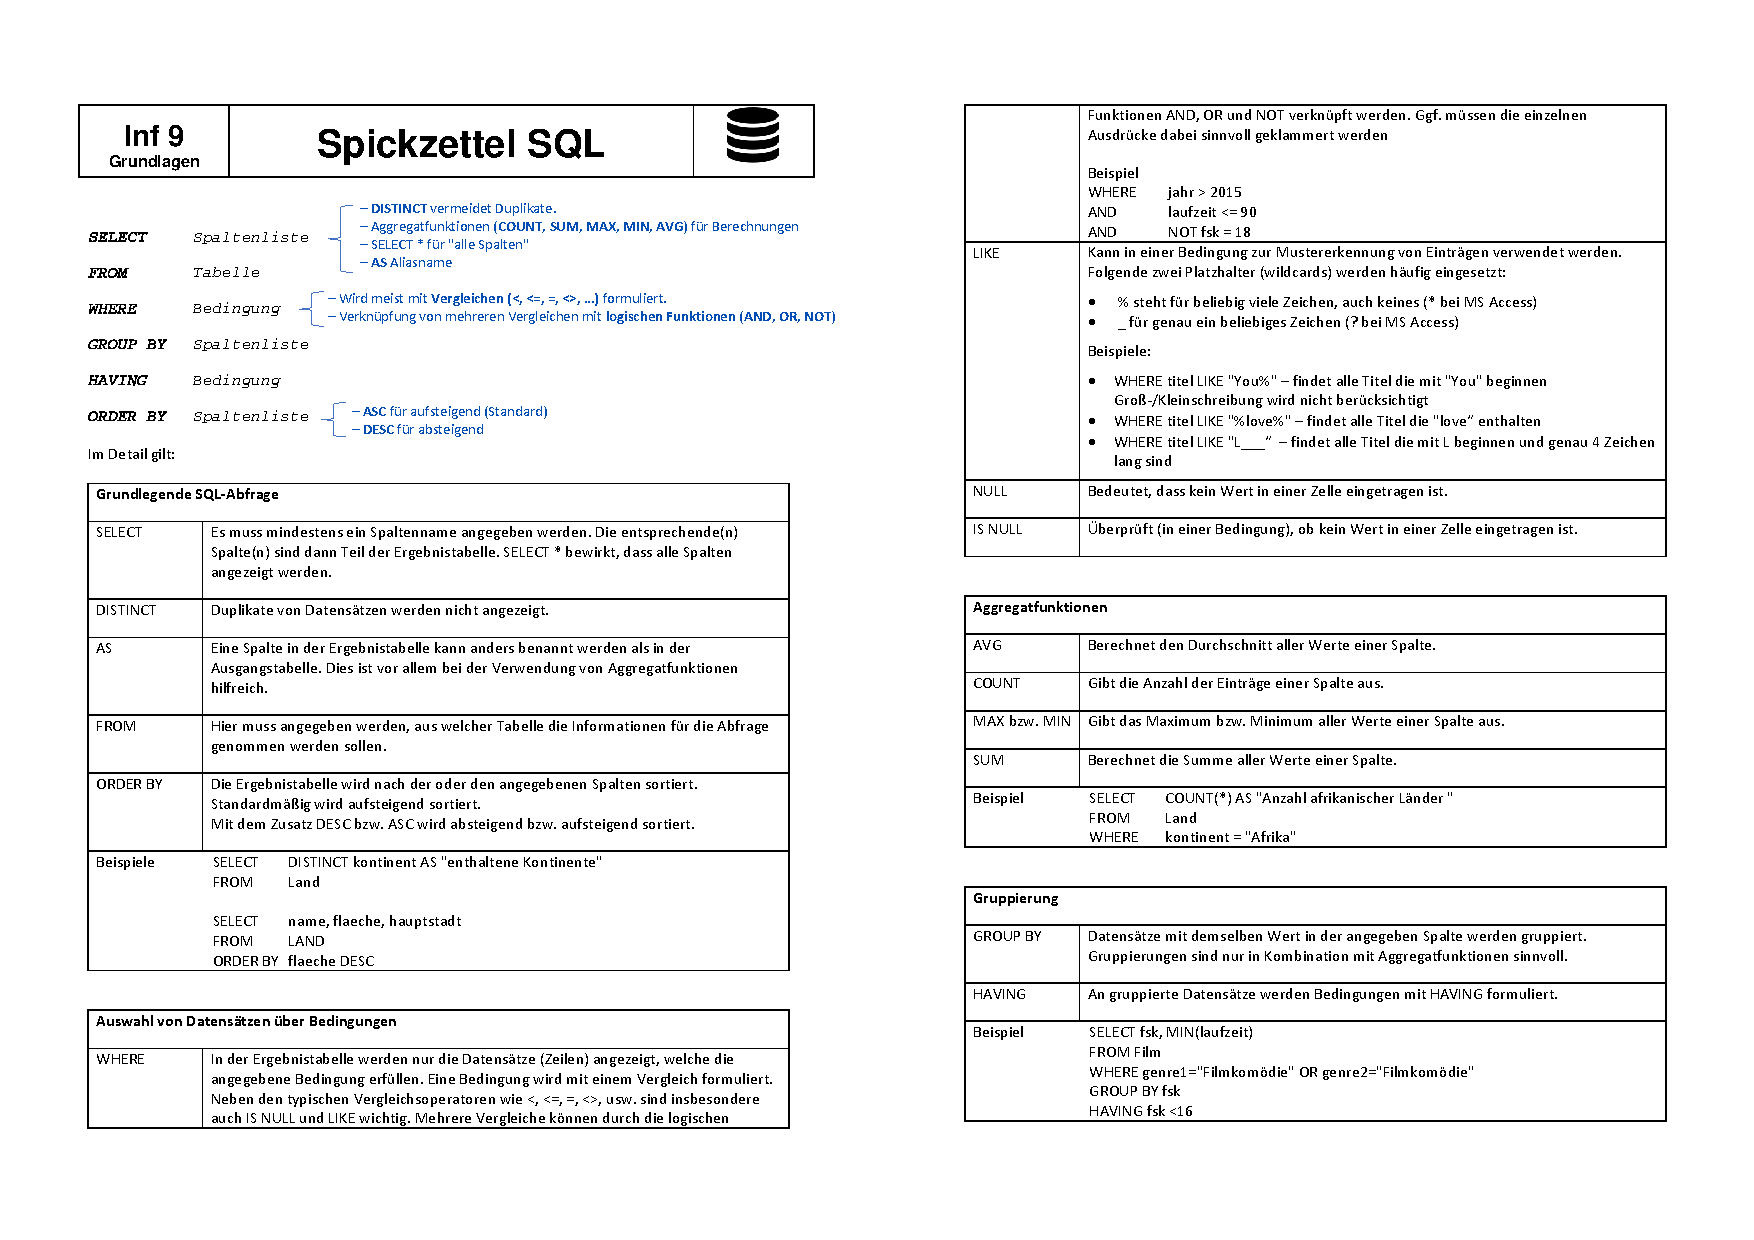
\includegraphics[width=\textwidth]{_Hefteintraege/img/SQL-Spickzettel_2on1.pdf}
        \fi
    \end{tcolorbox}
}
\newcommand{\sqlmemes}{
    \doppelseite{0.43}{0.5}{c}{
        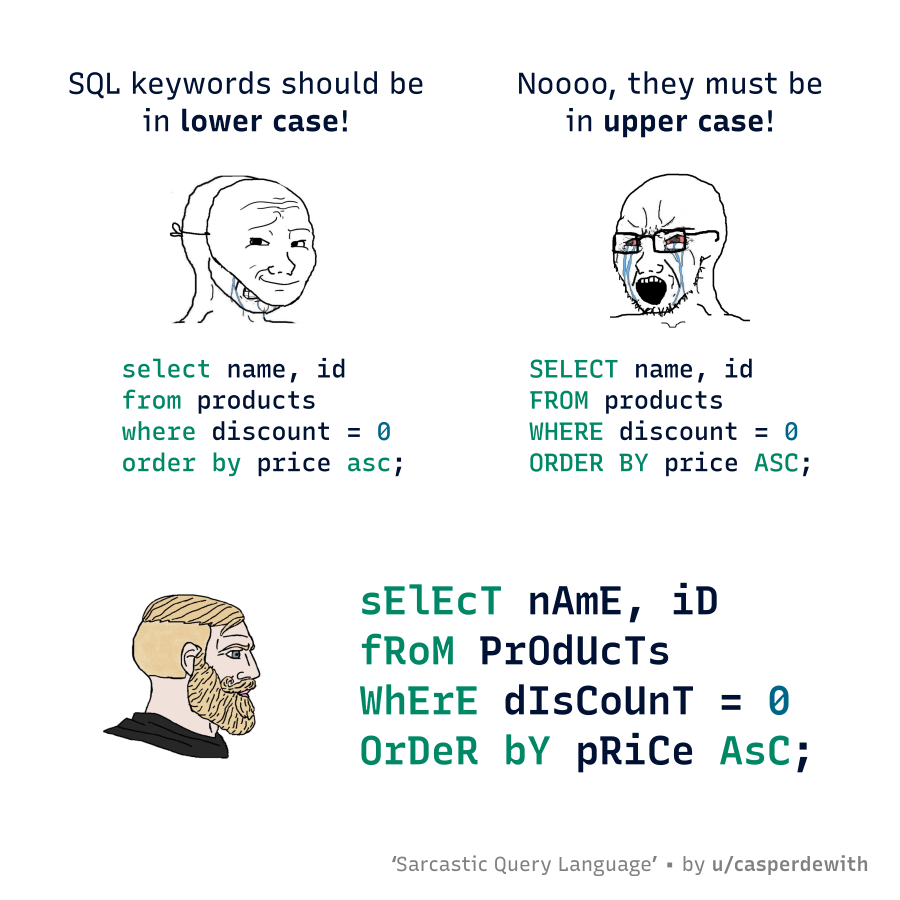
\includegraphics[width=\textwidth]{_Hefteintraege/img/sql_meme_1.png}
        
        \hinweis{SQL Schlüsselwörter wie SELECT, WHERE etc. sind nicht case-sensitive. Groß-/Kleinschreibung ist also egal.}
    }{
        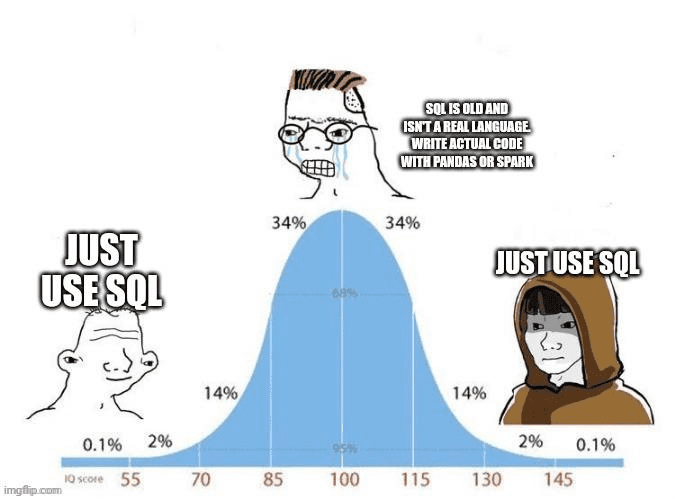
\includegraphics[width=\textwidth]{_Hefteintraege/img/sql_meme_2.png}
    }
}
\ifbeamer
\definesframe[false]{SQL Memes}{\sqlmemes}
\else
\sqlmemes
\fi

        \Aufgabe[25]{Übung: SQL Island}{
\UrlAndCode{sql-island.informatik.uni-kl.de/}
\begin{enumerate}
    \item Was sind die Primärschlüssel der Tabellen, die die einzelnen Objekte eindeutig identifizieren?
        \\$\rightarrow$ Notiert das vollständige Tabellenschema der Datenbank von SQL Island (mit Datentypen und Markierung der Primärschlüssel)\\
        \hinweis{Den Datentyp Character gibt es in den meisten Datenbanksystemen nicht. Wir verwenden daher immer String (=Text).}
        \\ \LoesungLine{{\fontfamily{pcr}\selectfont\footnotesize
                \textbf{BEWOHNER(\underline{int bewohnernr} , String name, int dorfnr, String geschlecht, String beruf, int gold, String status)}\\
                \textbf{GEGENSTAND(\underline{String gegenstand}, int besitzer)}\\
                \textbf{DORF(\underline{int dorfnr}, String name, int haeuptling)}
            }}{4}
    \item Stellt die Tabellen der Datenbank mit Klassenkarten dar.\\
    \vspace{0.2cm}
        \LoesungKaroTikz{
            \begin{class}{BEWOHNER}{0,0}
                \attribute{int bewohnernr}
                \attribute{String name}
                \attribute{int dorfnr}
                \attribute{String geschlecht}
                \attribute{String beruf}
                \attribute{int gold}
                \attribute{String status}
            \end{class}
            \begin{class}{GEGENSTAND}{6,0}
                \attribute{String gegenstand}
                \attribute{int besitzer}
            \end{class}
            \begin{class}{DORF}{12,0}
                \attribute{int dorfnr}
                \attribute{String name}
                \attribute{int haeuptling}
            \end{class}
        }{30}
    \item Spielt SQL Island, der SQL-Spickzettel hilft euch dabei.
\end{enumerate}

    



}

    }
    \mysession{Stunde 5+6}{
        % \ifbeamer
        %     \Aufgabe[25]{Übung: SQL Island}{
\UrlAndCode{sql-island.informatik.uni-kl.de/}
\begin{enumerate}
    \item Was sind die Primärschlüssel der Tabellen, die die einzelnen Objekte eindeutig identifizieren?
        \\$\rightarrow$ Notiert das vollständige Tabellenschema der Datenbank von SQL Island (mit Datentypen und Markierung der Primärschlüssel)\\
        \hinweis{Den Datentyp Character gibt es in den meisten Datenbanksystemen nicht. Wir verwenden daher immer String (=Text).}
        \\ \LoesungLine{{\fontfamily{pcr}\selectfont\footnotesize
                \textbf{BEWOHNER(\underline{int bewohnernr} , String name, int dorfnr, String geschlecht, String beruf, int gold, String status)}\\
                \textbf{GEGENSTAND(\underline{String gegenstand}, int besitzer)}\\
                \textbf{DORF(\underline{int dorfnr}, String name, int haeuptling)}
            }}{4}
    \item Stellt die Tabellen der Datenbank mit Klassenkarten dar.\\
    \vspace{0.2cm}
        \LoesungKaroTikz{
            \begin{class}{BEWOHNER}{0,0}
                \attribute{int bewohnernr}
                \attribute{String name}
                \attribute{int dorfnr}
                \attribute{String geschlecht}
                \attribute{String beruf}
                \attribute{int gold}
                \attribute{String status}
            \end{class}
            \begin{class}{GEGENSTAND}{6,0}
                \attribute{String gegenstand}
                \attribute{int besitzer}
            \end{class}
            \begin{class}{DORF}{12,0}
                \attribute{int dorfnr}
                \attribute{String name}
                \attribute{int haeuptling}
            \end{class}
        }{30}
    \item Spielt SQL Island, der SQL-Spickzettel hilft euch dabei.
\end{enumerate}

    



}
        % \fi

        \Aufgabe[15]{SQL Puzzle}{
    In dieser Aufgabe geht es immer um die Tabelle \emph{land}, deren erste Datensätze du hier siehst:

    \vspace{0.2cm}
    \begin{tabularx}{\textwidth}{C|C|C|C|C} 
       \emph{id} & \emph{name} & \emph{einwohner} & \emph{flaeche} & \emph{hauptstadt}\\\hline
       1 & Deutschland & 83.24 & 358 & Berlin \\
       2 & Frankreich & 67.39 & 544 & Paris \\
       3 & Brasilien & 212.60 & 8516 & Rio de Janeiro \\
       ... & ... & ... & ... & ... \\
    \end{tabularx}
    
    \setcounter{tmp}{1}

    \centering
    \emphColB{Welche SQL-Abfrage (rechte Seite) führt zu welcher Ergebnistabelle (linke Seite)? Ordne richtig zu!}

    \Loesung{
        Lösung:
        
        \begin{multicols}{3}
            \emphColB{\ShowAndStepCounter{tmp}{\arabic})} \emphColA{iv)} \pause
            
            \emphColB{\ShowAndStepCounter{tmp}{\arabic})} \emphColA{viii)} \pause
            
            \emphColB{\ShowAndStepCounter{tmp}{\arabic})} \emphColA{vii)} \pause
            
            \emphColB{\ShowAndStepCounter{tmp}{\arabic})} \emphColA{i)} \pause
            
            \emphColB{\ShowAndStepCounter{tmp}{\arabic})} \emphColA{ix)} \pause
            
            \emphColB{\ShowAndStepCounter{tmp}{\arabic})} \emphColA{iii)} \pause
            
            \emphColB{\ShowAndStepCounter{tmp}{\arabic})} \emphColA{v)} \pause
            
            \emphColB{\ShowAndStepCounter{tmp}{\arabic})} \emphColA{ii)} \pause
            
            \emphColB{\ShowAndStepCounter{tmp}{\arabic})} \emphColA{vi)}
        \end{multicols}
    }

    \ifbeamer
    \else
        \doppelseite{0.3}{0.3}{t}{
            \setcounter{tmp}{1}
            \begin{tabularx}{\textwidth}{C}\\
                \emphColB{\ShowAndStepCounter{tmp}{\arabic})}
                Zeige alle Spalten der Tabelle land.\\\\\hline\\
                \emphColB{\ShowAndStepCounter{tmp}{\arabic})}
                Zeige die Spalten name und hauptstadt der Tabelle land.\\\\\hline\\
                \emphColB{\ShowAndStepCounter{tmp}{\arabic})}
                Zeige die durchschnittliche Einwohnerzahl aller Länder.\\\\\hline\\
                \emphColB{\ShowAndStepCounter{tmp}{\arabic})}
                Zeige die Namen aller Länder in  alphabetisch absteigender Reihenfolge.\\\\\hline\\
                \emphColB{\ShowAndStepCounter{tmp}{\arabic})}
                Zeige die Hauptstädte der Länder, deren Einwohnerzahl größer als 50 Mio ist.\\\\\hline\\
                \emphColB{\ShowAndStepCounter{tmp}{\arabic})}
                Zeige die Anzahl aller Länder, deren Name mit 'land' endet. \\\\\hline\\
                \emphColB{\ShowAndStepCounter{tmp}{\arabic})}
                Zeige die Namen aller Länder, deren Fläche zwischen 100 und 999 Tausend km² liegt.\\\\\hline\\
                \emphColB{\ShowAndStepCounter{tmp}{\arabic})}
                Zeige die Namen der Länder, die mit 'D' beginnen oder mit 'd' aufhören. \\\\\hline\\
                \emphColB{\ShowAndStepCounter{tmp}{\arabic})}
                Zeige die Namen der drei Länder mit der größten Einwohnerzahl. \\
            \end{tabularx}
        }{
            \setcounter{tmp}{1}
            \begin{tabularx}{\textwidth}{C}
                \\
                \emphColA{\ShowAndStepCounter{tmp}{\roman})}
                SELECT name\\
                FROM land  \\
                ORDER BY name DESC;\\\\\hline\\
                \emphColA{\ShowAndStepCounter{tmp}{\roman})}
                SELECT name \\
                FROM land \\
                WHERE name LIKE 'D\%'  \\
                OR name LIKE '\%d';\\\\\hline\\
                \emphColA{\ShowAndStepCounter{tmp}{\roman})}
                SELECT COUNT(*) \\
                FROM land \\
                WHERE name LIKE '\%land';\\\\\hline\\
                \emphColA{\ShowAndStepCounter{tmp}{\roman})}
                SELECT * \\
                FROM land;\\\\\hline\\
                \emphColA{\ShowAndStepCounter{tmp}{\roman})}
                SELECT name  \\
                FROM land \\
                WHERE flaeche >= 100  \\
                AND flaeche <= 999;\\\\\hline\\
                \emphColA{\ShowAndStepCounter{tmp}{\roman})}
                SELECT name, einwohner \\
                FROM land  \\
                ORDER BY einwohner DESC \\
                LIMIT 3;\\\\\hline\\
                \emphColA{\ShowAndStepCounter{tmp}{\roman})}
                SELECT AVG(einwohner) \\
                FROM land; \\\\\hline\\
                \emphColA{\ShowAndStepCounter{tmp}{\roman})}
                SELECT name, hauptstadt \\
                FROM land;\\\\\hline\\
                \emphColA{\ShowAndStepCounter{tmp}{\roman})}
                SELECT hauptstadt \\
                FROM land \\
                WHERE einwohner > 50;
            \end{tabularx}
        }
    \fi
}


        \Aufgabe{\ifbeamer
\includegraphics[height=15pt]{_Aufgaben/img/artemis.png}~~~~\fi Wdh: SQL Basics}{
    Bearbeite die Aufgabe \emphColB{Wdh - SQL Basics} auf \url{artemis.tum.de}. Artemis gibt dir immer, wenn du auf Submit drückst, die ersten Zeilen der Ergebnistabelle und ob deine SQL-Abfrage (bzw. welche Teile von ihr) richtig sind, aus.
    
    Wenn du eine Abfrage richtig hast, notiere sie unten im Skript.
    
    Falls du bei Gruppierung und Aggregatfunktionen Schwierigkeiten hast, hilft dir dieses \emphColC{Video (bitte Kopfhörer verwenden!)}: \UrlAndCode{bycs.link/simpleclub-group-sort-aggregat}
    
    \setcounter{tmp}{1}
    
   \vspace{0.3cm} \emphColB{1)} 
   Vervollständige die SQL-Abfrage so, dass sie ID, Name, Art und URL aller Freibäder ausgibt.
    \\\LoesungKaro{SELECT id, name, art, url\\FROM Schwimmbad\\WHERE art='Freibad' }{6}
}
\UnterAufgabe{Wdh: SQL Basics}{
   \vspace{0.3cm} \emphColB{2)} 
   Schreibe eine SQL-Abfrage, die ausgibt, wie viele Gemeinden es im Regierungsbezirk 'Oberbayern' gibt. 
    \\\LoesungKaro{SELECT COUNT(*)\\FROM Gemeinde\\WHERE regierungsbezirk='Oberbayern'}{6}
   
   \vspace{0.3cm} \emphColB{3)} 
   Schreibe eine SQL-Abfrage, die Name, Straße und URL (also die Internetadresse) alle Zoos in der Gemeinde mit Schluessel '09162000' ausgibt.
    \\\LoesungKaro{SELECT name, strasse, url\\FROM Zoo\\WHERE gemeindeschluessel = '09162000'}{6}
}
   
\UnterAufgabe{Wdh: SQL Basics}{   
   \vspace{0.3cm} \emphColB{4)} 
   Schreibe eine SQL-Abfrage, die die Summe aller weiblichen Einwohnerinnen und die Summe aller männlichen Einwohner gruppiert nach Regierungsbezirk und den Namen des jeweiligen Regierungsbezirks ausgibt.
    \\\LoesungKaro{SELECT regierungsbezirk, SUM(einwohner\_w), SUM(einwohner\_m)\\FROM gemeinde\\GROUP BY regierungsbezirk}{6}
   
   \vspace{0.3cm} \emphColB{5)} 
   Schreibe eine SQL-Abfrage, die die durchschnittliche Fläche der Gemeinde eines Kreises (=Landkreis) und den Namen und Regierungsbezirk des jeweiligen Landkreises anzeigt. Sortiere die Ausgabe nach Name des Landkreises.
   \hinweis{Achtung: Du kannst bei der Verwendung von Gruppierung nur Spalten, nach denen gruppiert wird, und solche, die mit Aggregatfunktionen zusammengefasst werden, anzeigen! Überlege, wie du dieses Problem hier lösen kannst.}
    \\\LoesungKaro{SELECT regierungsbezirk, kreis, avg(flaeche)\\FROM Gemeinde\\GROUP BY regierungsbezirk,kreis\\ORDER BY kreis}{6}
}
   
\UnterAufgabe{Wdh: SQL Basics}{   
   \vspace{0.3cm} \emphColB{6)} 
   Schreibe eine SQL-Abfrage, die die Namen und Einwohnerzahlen aller Gemeinde, die mehr als 100.000 männliche und mehr als 100.000 weibliche Einwohner:innen haben, ausgibt.
    \\\LoesungKaro{SELECT name, einwohner\_m, einwohner\_w\\FROM Gemeinde\\WHERE einwohner\_m > 100000\\AND einwohner\_w > 100000}{6}
   
   \vspace{0.3cm} \emphColB{7)} 
   Schreibe eine SQL-Abfrage, die die Namen und Einwohnerzahlen aller Gemeinde, die mehr als 75.000 männliche oder mehr als 75.000 weibliche Einwohner:innen haben, ausgibt.
    \\\LoesungKaro{SELECT name, einwohner\_m, einwohner\_w \\FROM Gemeinde\\WHERE einwohner\_m > 75000\\OR einwohner\_w > 75000}{6}
}
   
\UnterAufgabe{Wdh: SQL Basics}{      
   \vspace{0.3cm} \emphColB{8)} 
   Schreibe eine SQL-Abfrage, die Name, Landkreis, Fläche und die Einwohnerzahlen aller Gemeinden ausgibt, die jeweils mehr als 50.000 männliche und weibliche Einwohner:innen oder eine Fläche größer als 100 km² hat.
    \\\LoesungKaro{SELECT name, kreis, flaeche, einwohner\_m, einwohner\_w\\FROM Gemeinde\\WHERE (einwohner\_m > 50000 AND einwohner\_w > 50000)\\OR flaeche > 100}{6}
   
   \vspace{0.3cm} \emphColB{9)} 
   Schreibe eine SQL-Abfrage, die die durchschnittlichen männlichen und weiblichen Einwohnerzahlen aller Gemeinde mit mehr als 100 km² Fläche pro Landkreis und den Namen des jeweiligen Landkreises ausgibt.
    \\\LoesungKaro{SELECT kreis, AVG(einwohner\_m), AVG(einwohner\_w)\\FROM Gemeinde\\WHERE flaeche > 100\\GROUP BY kreis}{6}
}
   
\UnterAufgabe{Wdh: SQL Basics}{      
   \vspace{0.3cm} \emphColB{10)} 
   Schreibe eine SQL-Abfrage, die die Anzahl von Wanderwegen, die zu einer Gemeinde führen in einer Spalte Anzahl und den jeweiligen Gemeindeschlüssel absteigend nach Anzahl sortiert, ausgibt.
    \\\LoesungKaro{SELECT gemeindeschluessel,COUNT(*) as Anzahl\\FROM Wanderweg\_zu\_Gemeinde\\GROUP BY gemeindeschluessel\\ORDER BY Anzahl DESC}{6}
}

    }
        
    \mysession{Stunde 7+8}{
        \Aufgabe[10]{Tabellenbeziehungen}{
    \begin{enumerate}
        \item Visualisiere (mit Bleistift), wer Häuptling in welchem Dorf ist.
        \item Überlege, wie du allgemein für diese zwei Tabellen darstellen kannst, wie sie (und ihre Spalten) miteinander in Beziehung stehen.
    \end{enumerate}

    \centering
    \ifbeamer\vspace{-1cm}\fi
    \begin{tikzpicture}
        \node[inner sep=0pt] (imgdorf01) at (1,1) {%
             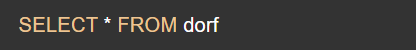
\includegraphics[width=0.25\textwidth]{_Aufgaben/img/A05/A05_Dorf_01.png}
        };
        \node[inner sep=0pt, below=-1pt of imgdorf01] (imgdorf02) {%
             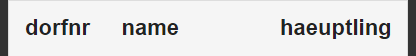
\includegraphics[width=0.25\textwidth]{_Aufgaben/img/A05/A05_Dorf_02.png}
        };
        \node[inner sep=0pt, below=-1pt of imgdorf02] (imgdorf03)  {%
             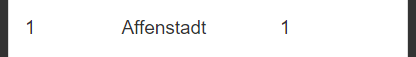
\includegraphics[width=0.25\textwidth]{_Aufgaben/img/A05/A05_Dorf_03.png}
        };
        \node[inner sep=0pt, below=-1pt of imgdorf03] (imgdorf04) {%
             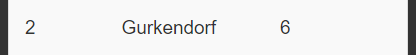
\includegraphics[width=0.25\textwidth]{_Aufgaben/img/A05/A05_Dorf_04.png}
        };
        \node[inner sep=0pt, below=-1pt of imgdorf04] (imgdorf05)  {%
             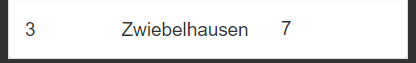
\includegraphics[width=0.25\textwidth]{_Aufgaben/img/A05/A05_Dorf_05b.png}
        };
        
        \node[inner sep=0pt, right = 2cm of imgdorf01] (imgbew01) {%
             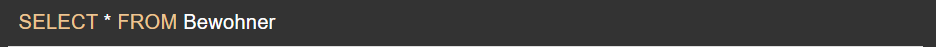
\includegraphics[width=0.55\textwidth]{_Aufgaben/img/A05/A05_Bew_01.png}
        };
        \node[inner sep=0pt, below=-1pt of imgbew01] (imgbew02) {%
             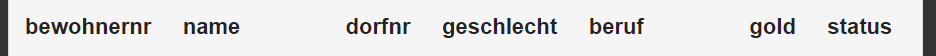
\includegraphics[width=0.55\textwidth]{_Aufgaben/img/A05/A05_Bew_02.png}
        };
        \node[inner sep=0pt, below=-1pt of imgbew02] (imgbew03) {%
             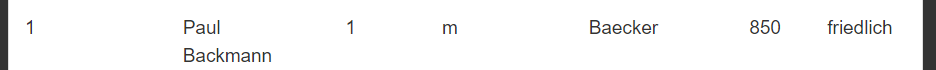
\includegraphics[width=0.55\textwidth]{_Aufgaben/img/A05/A05_Bew_03.png}
        };
        \node[inner sep=0pt, below=-1pt of imgbew03] (imgbew04) {%
             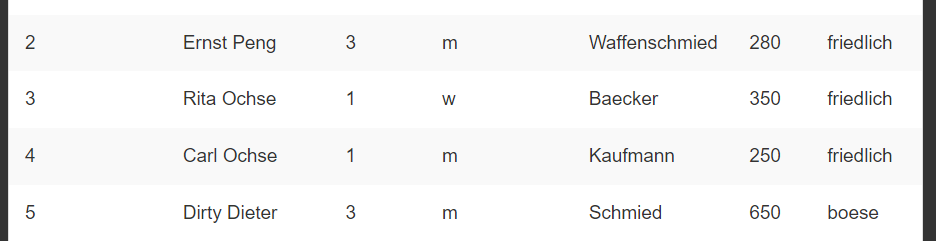
\includegraphics[width=0.55\textwidth]{_Aufgaben/img/A05/A05_Bew_04.png}
        };
        \node[inner sep=0pt, below=-1pt of imgbew04] (imgbew05) {%
             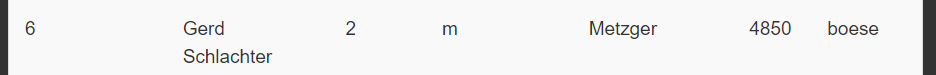
\includegraphics[width=0.55\textwidth]{_Aufgaben/img/A05/A05_Bew_05.png}
        };
        \node[inner sep=0pt, below=-1pt of imgbew05] (imgbew06) {%
             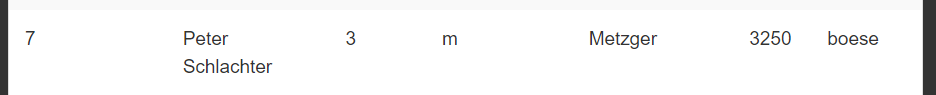
\includegraphics[width=0.55\textwidth]{_Aufgaben/img/A05/A05_Bew_06b.png}
        };
        \node[inner sep=0pt, below=-1pt of imgbew06] (imgbew07) {%
             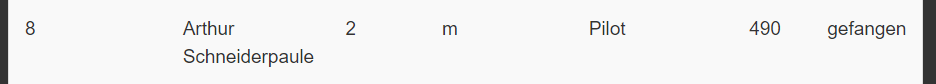
\includegraphics[width=0.55\textwidth]{_Aufgaben/img/A05/A05_Bew_07b.png}
        };
        %\Loesung{\draw[arrow] (imgdorf02) -- (imgbew02);}
        \Loesung{\draw[-{angle 60}, colA] (imgdorf03.east) to[out=0, in=180] (imgbew03.west);}
        \Loesung{\draw[-{angle 60}, colB] (imgdorf04.east) to[out=0, in=180] (imgbew05.west);}
        \Loesung{\draw[-{angle 60}, colC] (imgdorf05.east) to[out=0, in=180] (imgbew06.west);}
        \Loesung{\draw[-{angle 60}, red] (imgdorf02.north east) ++(-1cm, 0) to[out=45, in=180] (imgbew02.west) ;}
        \Loesung{\draw[-{angle 60}, red] (imgbew02.north) ++(-1cm, 0) to[out=150, in=25] ([shift={(-1.5cm, 0)}]imgdorf02.north);}

        %\node[above left = 0pt and 1pt of imgbew02, red] {1};
    \end{tikzpicture}
    
}

\UnterAufgabe[10]{Tabellenbeziehung im Klassendiagramm}{
    \ifbeamer\else\emphColB{Tabellenbeziehung im Klassendiagramm}\fi
    \begin{enumerate}
        \item Ergänze das Klassendiagramm entsprechend der beiden Tabellen oben.
        \item Wie kann man die Beziehungen zwischen den beiden Tabellen im Klassendiagramm darstellen?\\
            Tipp: Unsere Überlegungen von oben, helfen dabei.
    \end{enumerate}

{
    \ifloesung 
        %\color{\LFarbe}
        \renewcommand{\umldrawcolor}{\LFarbe}
        \renewcommand{\umltextcolor}{\LFarbe}
        \fontspec{Comic Sans MS} 
    \fi
    \begin{tikzpicture}
        \begin{class}[text width=7cm]{Dorf}{0,-1}
            \attribute{\ifloesung int dorfnr\fi}
            \attribute{\ifloesung String name\fi}
            \attribute{}
            \attribute{}
            \attribute{}
            \attribute{}
        \end{class}
        \begin{class}[text width=7cm]{Bewohner}{11,0}
            \attribute{\ifloesung int bewohnernr\fi}
            \attribute{\ifloesung String name\fi}
            \attribute{\ifloesung String geschlecht\fi}
            \attribute{\ifloesung String beruf\fi}
            \attribute{\ifloesung int gold\fi}
            \attribute{\ifloesung String status\fi}
            \attribute{}
            \attribute{}
            \attribute{}
            \attribute{}
            \attribute{}
        \end{class}
        \Loesung{\unidirectionalAssociation{Dorf}{1}{haeuptling}{Bewohner}}
    \end{tikzpicture}
    
    \renewcommand{\umldrawcolor}{\TFarbe}
    \renewcommand{\umltextcolor}{\TFarbe}
    }
}

    
        \Hefteintrag{1.8}{Tabellenbeziehungen: Fremdschlüssel}{
    Wenn Datensätze mittels Primärschlüssel in einer anderen Tabelle verwendet werden, spricht man dort von einem Fremdschlüssel. Im \emphColA{Tabellenschema} werden die \emphColA{\LoesungLuecke{Fremdschlüssel}{8cm}} durch \emphColA{$\overline{\textbf{\LoesungLeer{"uberstreichen}{8cm}}}$} (manchmal auch \emphColA{\dotuline{\LoesungLeer{unterpunkten}{8cm}}}) markiert. Ein Beispiel in SQL-Island ist der Häuptling eines Dorfes, der in der Tabelle Dorf mittels bewohnernr eingetragen wird. Die \emphColB{bewohnernr} ist hierbei \emphColB{\LoesungLuecke{Primärschlüssel}{8cm}} in der \emphColB{Tabelle Bewohner} und \emphColC{\LoesungLuecke{Fremdschlüssel}{8cm}} in der \emphColC{Tabelle Dorf} (heißt hier aber \emphColC{haeuptling}).

}


    }
        
    \mysession{Stunde 9+10}{

        \Hefteintrag{1}{Tabellenbeziehungen im Klassendiagramm}{
    \ifbeamer\else\vspace{12pt}\fi
    \LoesungLeer{}{2cm}
    \begin{tikzpicture}
        \begin{class}{TabelleA}{0,0}
            \attribute{int id}
            \attribute{String spalte1}
            \attribute{...}
        \end{class}
        \begin{class}{TabelleB}{11,0}
            \attribute{int id}
            \attribute{String spalte1}
            \attribute{...}
        \end{class}
        
        \Loesung{\uniAssociation{TabelleA}{n}{{fremdschlüssel}}{1}{TabelleB}}
    \end{tikzpicture}

    \LoesungLeer{{
    
        \begin{itemize}
        \color{\LFarbe}
            \item Beziehungspfeil immer vom Fremd- zum Primärschlüssel.
            \item 'fremdschluessel' ist eine Spalte der TabelleA, wird dort aber nicht eingetragen.
            \item Die Form der Pfeilspitze ist wichtig und muss genau so sein, da andere Spitzen andere Bedeutungen haben!
            \item Kardinalität an der Pfeilspitze ist immer 1 (bei Datenbanken), da in einer Spalte (eines Datensatzes) immer nur ein Wert stehen kann. 
        \end{itemize}
    }}{2cm}
}

        \input{_Hefteintraege/H05_Kardinalität}

        \Aufgabe[15]{\ifbeamer
\includegraphics[height=15pt]{_Aufgaben/img/artemis.png}~~~~\fi Klassendiagramm Flugverspätung}{

Bearbeite diese Aufgabe auf \url{artemis.tum.de}.

Erstelle ein Klassendiagramm für die Datenbank unter \UrlAndCode{dbiu.de/flugverspaetungen/}.

Damit du weniger schreiben musst, kannst du die \emphColB{letzten 6} Spalten der \emphColB{Tabelle Flug} durch \emphColB{... ersetzen}.

Achte auf korrektes Format, Datentypen und Kardinalitäten. Zeichne das Diagramm anschließend unten auf:

\LoesungKaroTikz{
    \begin{class}{Flughafen}{0,0}
        \attribute{int id}
        \attribute{String land}
        \attribute{String ort}
        \attribute{String name}
    \end{class}
    
    \begin{class}{Flug}{5,4}
        \attribute{int id}
        \attribute{DATUM datum}
        \attribute{int flugnr}
        \attribute{String flugzeug}
        \attribute{...}
    \end{class}
    
    \begin{class}{Fluggesellschaft}{12,4}
        \attribute{String id}
        \attribute{String name}
    \end{class}

    \uniAssociationAngle{Flug.west}{180}{above}{n}{startflughafen}{1}{left}{90}{Flughafen.north}
    \uniAssociationAngle{Flug.south}{270}{right}{n}{zielflughafen}{1}{below}{0}{Flughafen.east}
    
    \uniAssociationAngle{Flug.east}{320}{below}{n}{fluggesellschaft$\_$id}{1}{below}{270}{Fluggesellschaft.south}
}{20}

}

        \Aufgabe{SQL: Tabellen verbinden}{
    Wir kennen jetzt Tabellen, die miteinander über Fremd- und Primärschlüssel in Beziehung stehen. Nun möchten wir aus diesen Tabellen auch zusammengehörende Datensätze abfragen.

    Öffne dafür \UrlAndCode{www.dbiu.de/flugverspaetungen} und führe folgende SQL-Abfrage aus:

    \begin{center}
        \emphColB{
        SELECT *\\
        FROM Fluggesellschaft, Flug}
    \end{center}

}

\ifbeamer
\definesframe[false]{}{
    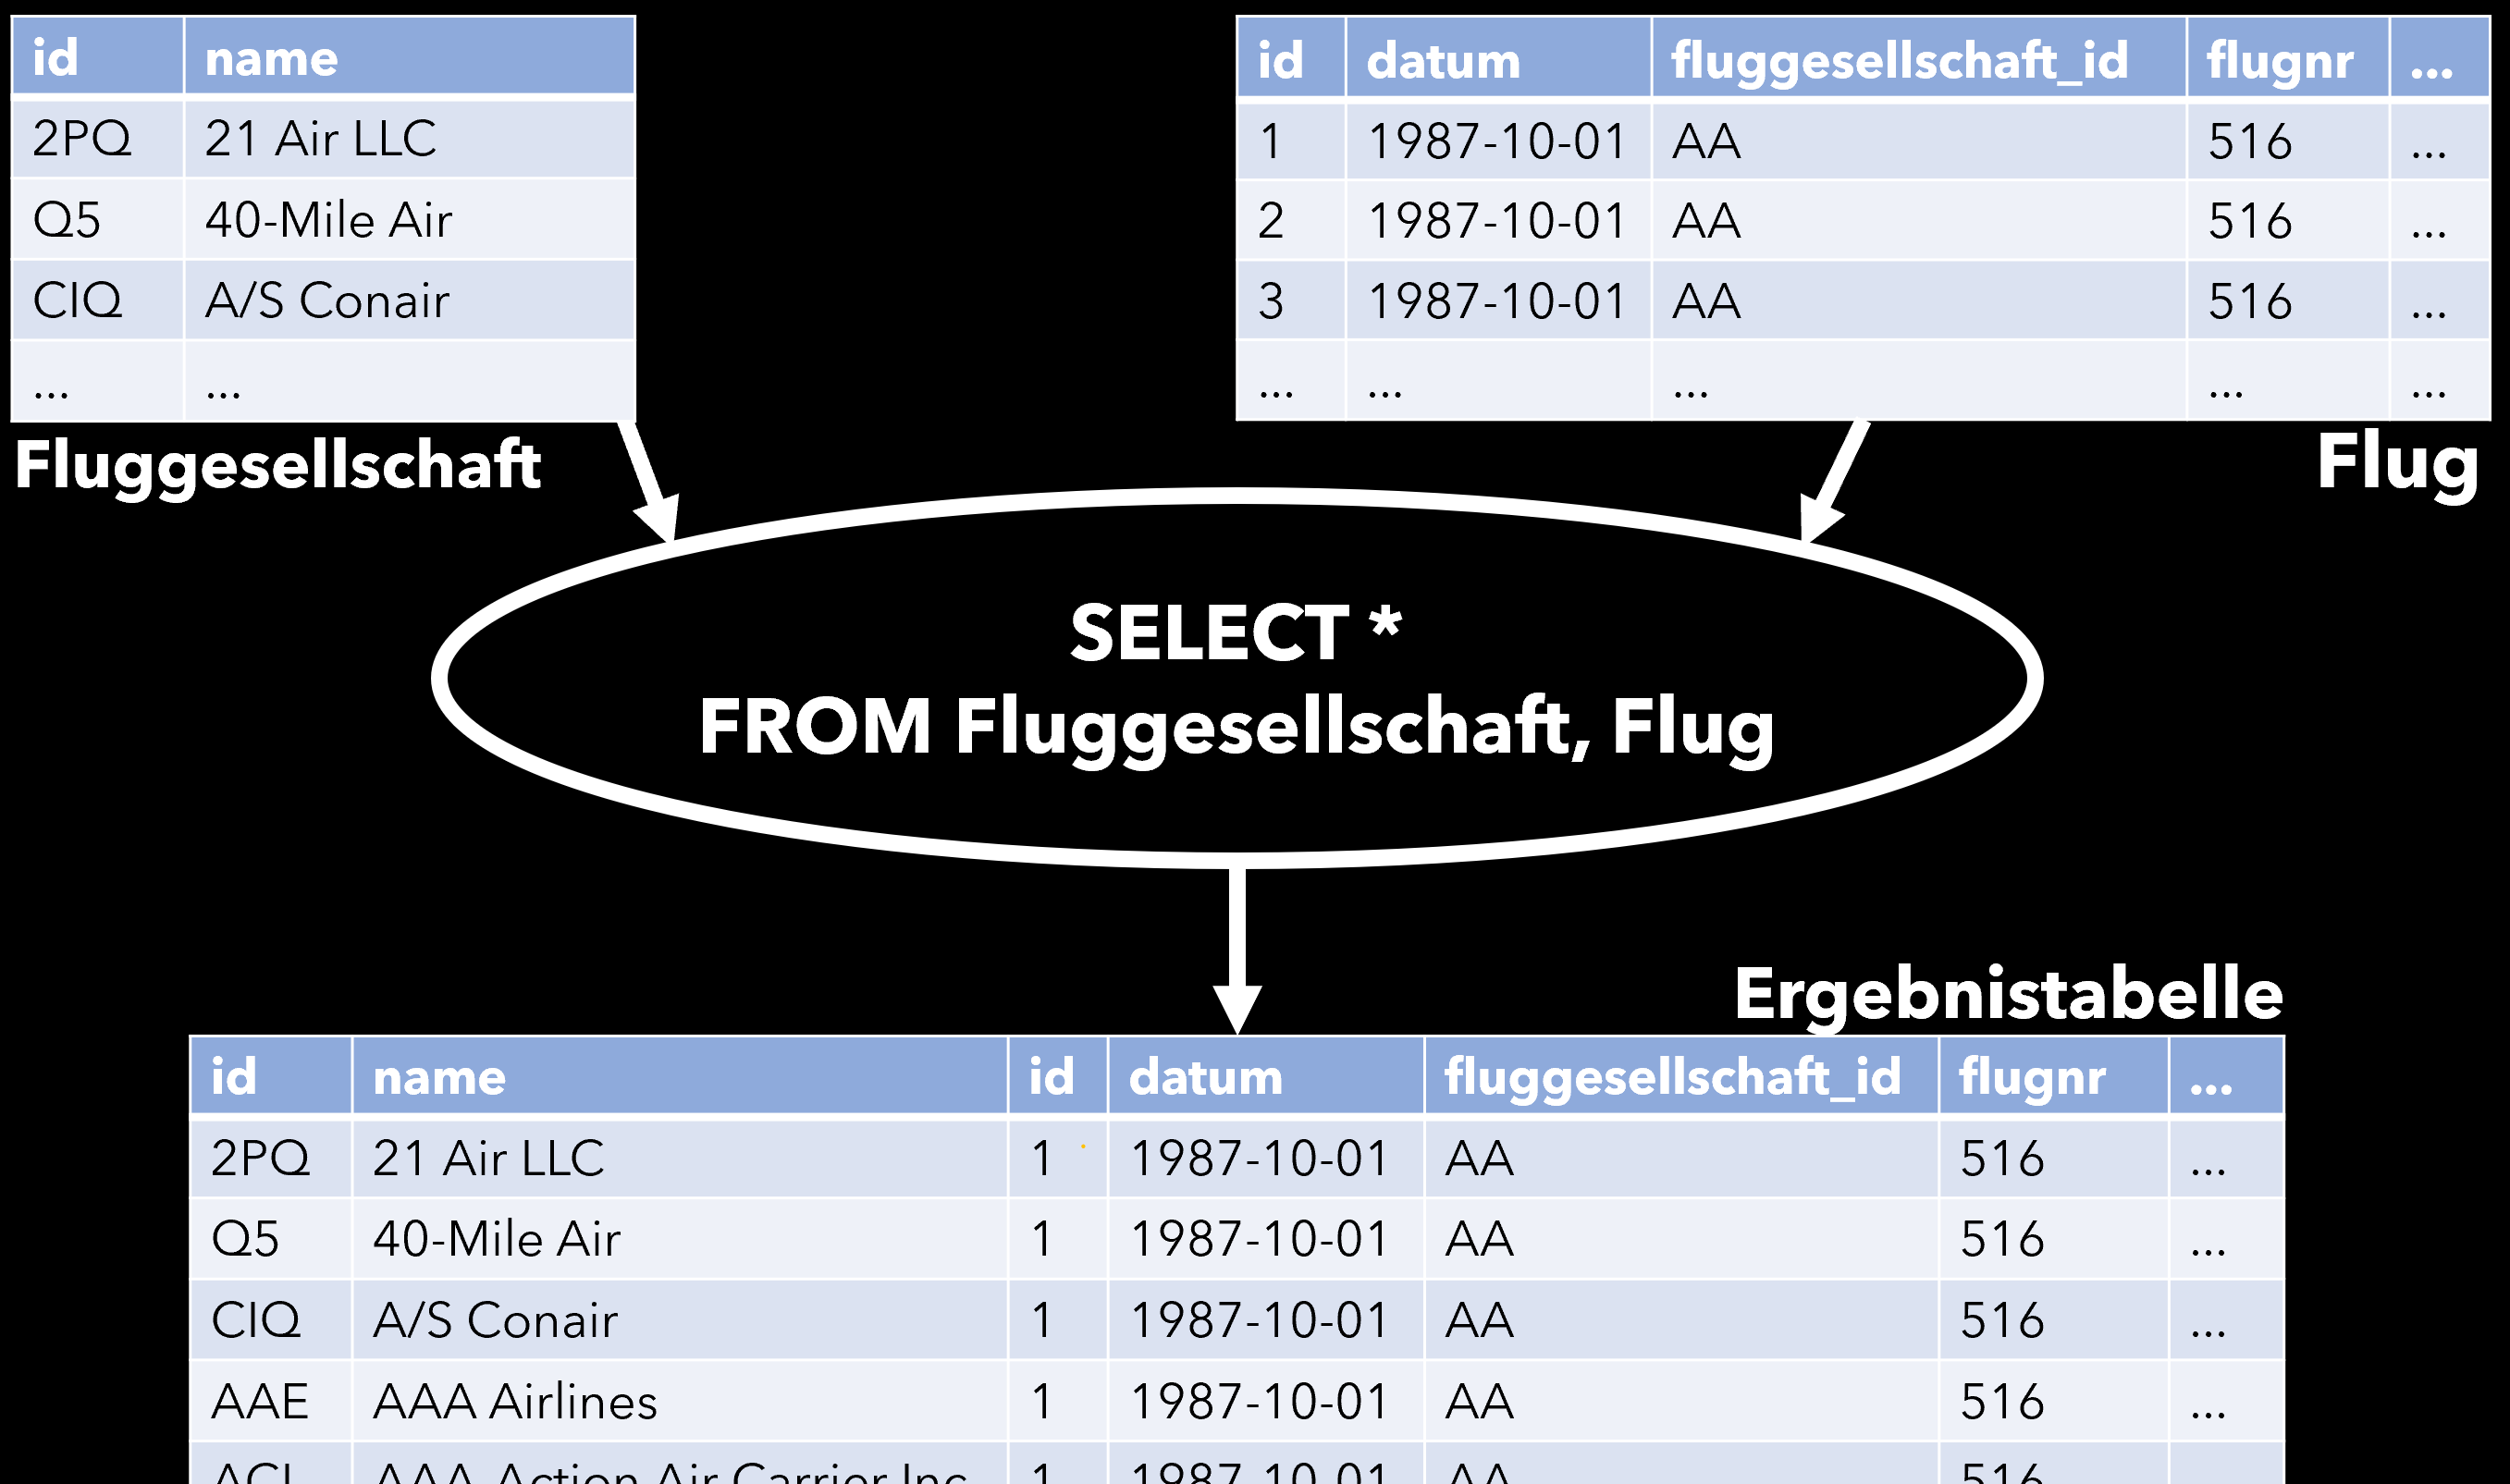
\includegraphics[height=\pageheight]{_Aufgaben/img/A07_Abfrage.png}
}
\fi

\UnterAufgabe{SQL: Tabellen verbinden}{

    Was beobachtest du? Werden nur zusammengehörende Datensätze angezeigt? Falls nicht, nach welchem Muster werden die beiden Tabellen miteinander kombiniert?

    \LoesungLine{Nein, es werden alle Datensätze aus einer mit allen Datensätzen aus der anderen kombiniert und die Spalten einfach hintereinander aufgereiht.}{3}
}

        \Hefteintrag{1.7}{Kreuzprodukt / Join}{
Möchte man Daten aus zwei Tabellen mit Beziehung zueinander abfragen, gibt man beide Tabellen \emphColA{mit Komma getrennt nach FROM} an.

Die SQL-Abfrage bildet dann das \LoesungLuecke{Kreuzprodukt}{7cm} der Tabellen. Die Ergebnistabelle enthält \LoesungLuecke{alle Kombinationen}{7cm} von Datensätzen beider Tabellen \emphColA{(Merkregel: \LoesungLuecke{Jeder mit Jedem}{9cm})}.

Um nur zusammengehörige Datensätze (also solche, die miteinenader in Beziehung stehen, z.B. eine Bewohner mit seinem Dorf) auszuwählen, ergänzt man als \emphColC{Selektion} eine \emphColC{Gleichheitsbedingung} zwischen Fremd- und zugehörigem \LoesungLuecke{Primärschlüssel}{8cm}. Dann spricht man von einem \LoesungLuecke{Join}{4cm}.

Zum Beispiel kann man in SQL-Island die Daten aller Dörfer und ihrer zugehörigen Häuptlinge so ausgeben:



\begin{center}
SELECT * \\\emphColA{FROM Dorf, Bewohner} \\\emphColC{WHERE Dorf.haeuptling = Bewohner.bewohnernr}    
\end{center}
}

    }
    
     \mysession{Stunde 11+12}{
         \Hefteintrag{1}{Join Beispiel}{
\ifbeamer\else\vspace{0.3cm}\fi
\centering
\begin{minipage}[t]{0.25\textwidth}
    \centering
    Lehrkraft\\\vspace{0.1cm}
    \begin{tabular}{c|c|c}
        id & kuerzel & schule \\\hline
        1 & Her & MTG\\
        2 & Ext & Dante\\
    \end{tabular}
\end{minipage}
\hfill
\begin{minipage}[t]{0.45\textwidth}
    \centering
    \emphColB{SELECT * \\FROM Lehrkraft, Schule}\\
    \emphColC{WHERE Lehrkraft.schule = Schule.id}
\end{minipage}
\hfill
\begin{minipage}[t]{0.25\textwidth}
    \centering
    Schule\\\vspace{0.1cm}
    \begin{tabular}{c|c}
        id & ort \\\hline
        MTG & Haidh.\\
        Dante & Sendl.\\
    \end{tabular}\
\end{minipage}

\vspace{0.2cm}
\emphColB{Ergebnistabelle des Kreuzprodukts:}\\\vspace{0.1cm}
\begin{tabular}{c|c|c|c|c}
    id & kuerzel & schule & id & ort \\\hline
    1 & Her & \emphColC{MTG} & \emphColC{MTG} & Haidh. \\
    2 & Ext & \emphColor{red}{Dante} & \emphColor{red}{MTG} & Haidh. \\
    1 & Her & \emphColor{red}{MTG} & \emphColor{red}{Dante} & Sendl. \\ 
    2 & Ext & \emphColC{Dante} & \emphColC{Dante} & Sendl.\\
\end{tabular}

\vspace{0.5cm}
\emphColC{Ergebnistabelle des Joins}\\\vspace{0.1cm}
\begin{tabular}{c|c|c|c|c}
    id & kuerzel & schule & id & ort \\\hline
    1 & Her & \emphColC{MTG} & \emphColC{MTG} & Haidh. \\
    2 & Ext & \emphColC{Dante} & \emphColC{Dante} & Sendl.\\
\end{tabular}

}
    
        \Aufgabe[45]{\ifbeamer
\includegraphics[height=15pt]{_Aufgaben/img/artemis.png}~~~~\fi SQL mit Kreuzprodukt und Join}{

Bearbeite diese Aufgabe auf \url{artemis.tum.de}. Du bekommst eine automatische Rückmeldung, ob deine Abgabe korrekt ist.
Alle Aufgaben beziehen sich auf die Datenbank mit untem stehendem Klassendiagramm. Eine Online-Version gibt es unter \url{www.dbiu.de/bayern/}, dort ist auch das Tabellenschema zu finden.

Gib immer genau die geforderten Daten aus und nicht mehr. Sortiere nicht, wenn du nicht dazu aufgefordert wirst.

\emphColB{Notiere unten anschließend deine korrekten SQL-Abfragen unten.}

}

\UnterAufgabe{\ifbeamer
\includegraphics[height=15pt]{_Aufgaben/img/artemis.png}~~~~\fi SQL mit Kreuzprodukt und Join}{
% TODO: Ersetzen
\begin{center}
% \ifbeamer
%     \includegraphics[width=0.6\textwidth]{img/Bayern_DB.png}
% \else
%     \includegraphics[width=\textwidth]{img/Bayern_DB.png}
% \fi


\begin{tikzpicture}
    \begin{class}{Gemeinde}{0,0}
        \attribute{String schluessel}
        \attribute{String regierungsbezirk}
        \attribute{String kreis}
        \attribute{String name}
        \attribute{String zusatz}
        \attribute{String plz}
        \attribute{float flaeche}
        \attribute{int einwohner$\_$m}
        \attribute{int einwohner$\_$w}
    \end{class}
    \begin{class}{Freizeitpark}{-6.5,3}
        \attribute{int id}
        \attribute{String name}
        \attribute{String strasse}
        \attribute{String url}
        \attribute{float breitengrad}
        \attribute{float laengengrad}
    \end{class}
    \begin{class}{Schwimmbad}{6.5,3}
        \attribute{int id}
        \attribute{String name}
        \attribute{String art}
        \attribute{String strasse}
        \attribute{String url}
        \attribute{float breitengrad}
        \attribute{float laengengrad}
    \end{class}
    \begin{class}{Radweg}{0,3}
        \attribute{String radweg$\_$id}
        \attribute{String name}
    \end{class}
    \begin{class}{Wanderweg}{6.5,-4.2}
        \attribute{String wanderweg$\_$id}
        \attribute{String name}
    \end{class}
    \begin{class}{Zoo}{-6.5,-2.5}
        \attribute{int id}
        \attribute{String name}
        \attribute{String strasse}
        \attribute{String url}
        \attribute{float breitengrad}
        \attribute{float laengengrad}
    \end{class}
    
    \uniAssociationAngle
    {Freizeitpark.south}{270}
    {left}{n}
    {gemeindeschluessel}
    {1}{below}
    {180}{[shift={(0,1.5)}]Gemeinde.west}
    
    \uniAssociationAngle
    {Schwimmbad.south}{270}
    {right}{n}
    {gemeindeschluessel}
    {1}{below}
    {0}{[shift={(0,1.3)}]Gemeinde.east}
    
    
    \uniAssociationAngle
    {[shift={(0,0)}]Zoo.south east}{0}
    {right}{n}
    {gemeindeschluessel}
    {1}{below}
    {180}{[shift={(0,0)}]Gemeinde.south west}
    
    \biAssociationAngle
    {[shift={(2.5,0)}]Radweg.south}{270}
    {left}{n}
    {Radweg$\_$zu$\_$Gemeinde}
    {m}{left}
    {90}{[shift={(2,0)}]Gemeinde.north}
    
    \biAssociationAngle
    {[shift={(-1,0)}]Wanderweg.north}{90}
    {right}{n}
    {Wanderweg$\_$zu$\_$Gemeinde}
    {m}{above}
    {0}{[shift={(0,-1)}]Gemeinde.east}
    
    \biAssociationAngle
    {[shift={(1.7,0)}]Gemeinde.south}{270}
    {left}{n}
    {Nachbargemeinde}
    {m}{right}
    {270}{[shift={(-0.1,0)}]Gemeinde.south east}
\end{tikzpicture}


\end{center}
}

\UnterAufgabe{\ifbeamer
\includegraphics[height=15pt]{_Aufgaben/img/artemis.png}~~~~\fi SQL mit Kreuzprodukt und Join}{
Verändere die SQL-Abfrage so, dass die Namen und Internetadressen (=url) aller Zoos und der Name und Regierungsbezirk der jeweiligen Gemeinde ausgegeben wird:

\vspace{0.3cm}

\large
\emphColB{SELECT Zoo.name, Gemeinde.name} \LoesungLuecke{,Gemeinde.regierungsbezirk, Zoo.url}{8cm}

\vspace{0.5cm}
\emphColB{FROM Zoo, Gemeinde}

\vspace{0.5cm}
\LoesungLuecke{WHERE Zoo.gemeindeschluessel = Gemeinde.schluessel}{17cm}

}

\UnterAufgabe{\ifbeamer
\includegraphics[height=15pt]{_Aufgaben/img/artemis.png}~~~~\fi SQL mit Kreuzprodukt und Join}{

Verändere die SQL-Abfrage so, dass die Namen und Straßen aller Freizeitparks und die Namen der jeweils zugehörigen Gemeinde ausgegeben wird.

\vspace{0.3cm}
\large
\emphColB{SELECT Freizeitpark.name, Gemeinde.name} \LoesungLuecke{, Freizeitpark.strasse}{8cm}

\vspace{0.5cm}
\emphColB{FROM Freizeitpark, Gemeinde}

\vspace{0.5cm}
\LoesungLuecke{WHERE Gemeinde.schluessel = Freizeitpark.gemeindeschluessel}{17cm}

}

\UnterAufgabe{\ifbeamer
\includegraphics[height=15pt]{_Aufgaben/img/artemis.png}~~~~\fi SQL mit Kreuzprodukt und Join}{
Schreibe eine SQL-Abfrage, die Namen und Art aller Schwimmbäder und den Namen und alle Einwohnerzahlen der zugehörigen Gemeinden ausgibt.

\LoesungKaro{SELECT Schwimmbad.name, Schwimmbad.art, \\ Gemeinde.name, Gemeinde.einwohner$\_$m, Gemeinde.einwohner$\_$w\\
FROM Schwimmbad, Gemeinde\\
WHERE Gemeinde.schluessel = Schwimmbad.gemeindeschluessel}{8}
}

\UnterAufgabe{\ifbeamer
\includegraphics[height=15pt]{_Aufgaben/img/artemis.png}~~~~\fi SQL mit Kreuzprodukt und Join}{

Schreibe eine SQL-Abfrage, die die Anzahl an Schwimmbädern in Gemeinden mit \emph{mehr} als 1000 weiblichen Einwohnerinnen ausgibt.

\emph{Tipp: Hier brauchst du mehrere verknüpfte Bedingungen}

\LoesungKaro{SELECT COUNT(*)\\
FROM Schwimmbad, Gemeinde\\
WHERE Gemeinde.schluessel = Schwimmbad.gemeindeschluessel\\
  AND Gemeinde.einwohner$\_$w > 1000}{8}
}

\UnterAufgabe{\ifbeamer
\includegraphics[height=15pt]{_Aufgaben/img/artemis.png}~~~~\fi SQL mit Kreuzprodukt und Join}{
Schreibe eine SQL-Abfrage, die die Namen aller Gemeinde in Oberbayern oder Niederbayern, zu denen ein Wanderweg führt, ausgibt. Dopplungen dürfen auftreten und sollte nicht entfernt werden!

\emph{Tipp: Hier brauchst du wieder mehrere verknüpfte Bedingungen. Überlege bei der Verknüpfung von Bedingungen, ob du Klammern setzen musst!}

\LoesungKaro{SELECT Gemeinde.name\\
FROM Gemeinde,Wanderweg$\_$zu$\_$Gemeinde\\
WHERE Gemeinde.schluessel = Wanderweg$\_$zu$\_$Gemeinde.gemeindeschluessel\\
AND (Gemeinde.regierungsbezirk='Oberbayern' \\
OR Gemeinde.regierungsbezirk='Niederbayern')}{10}
}

\UnterAufgabe{\ifbeamer
\includegraphics[height=15pt]{_Aufgaben/img/artemis.png}~~~~\fi SQL mit Kreuzprodukt und Join}{
Schreibe eine SQL-Abfrage, die aus den Tabellen Gemeinde und Wanderweg$\_$zu$\_$Gemeinde die Anzahl der Wanderwege, die zu Gemeinden mit mehr als 500 000 männlichen Einwohnern führen, ausgibt.


\LoesungKaro{SELECT COUNT(*)\\
FROM Gemeinde, Wanderweg$\_$zu$\_$Gemeinde\\
WHERE Gemeinde.schluessel = Wanderweg$\_$zu$\_$Gemeinde.gemeindeschluessel\\
  AND einwohner$\_$m > 500000}{8}
}

\UnterAufgabe{\ifbeamer
\includegraphics[height=15pt]{_Aufgaben/img/artemis.png}~~~~\fi SQL mit Kreuzprodukt und Join}{
Schreibe eine SQL-Abfrage, die eine Liste mit den Namen aller Gemeinden, die ein 'Freibad' haben, und die Namen der jeweiligen Freibäder ausgibt. 

\LoesungKaro{SELECT Gemeinde.name, Schwimmbad.name\\
FROM Gemeinde, Schwimmbad\\
WHERE Gemeinde.schluessel=Schwimmbad.gemeindeschluessel\\
AND Schwimmbad.art='Freibad'}{8}
}

\UnterAufgabe{\ifbeamer
\includegraphics[height=15pt]{_Aufgaben/img/artemis.png}~~~~\fi SQL mit Kreuzprodukt und Join}{
Schreibe eine SQL-Abfrage, die die Anzahl an Radwegen, die an Gemeinden im PLZ-Bereich \emphColA{größer} als 96400 angrenzen, ausgibt.

\LoesungKaro{SELECT COUNT(*)\\
FROM Gemeinde, Radweg$\_$zu$\_$Gemeinde\\
WHERE Gemeinde.schluessel=Radweg$\_$zu$\_$Gemeinde.gemeindeschluessel\\
  AND Gemeinde.plz > 96400}{8}

}

\UnterAufgabe{\ifbeamer
\includegraphics[height=15pt]{_Aufgaben/img/artemis.png}~~~~\fi SQL mit Kreuzprodukt und Join}{
\begin{minipage}[t]{\textwidth}
Schreibe eine SQL-Abfrage, die die Namen aller Zoos in einer Gemeinde namens 'Erlangen' ausgibt.

\LoesungKaro{SELECT Zoo.name\\
FROM Zoo,Gemeinde\\
WHERE Zoo.gemeindeschluessel = Gemeinde.schluessel\\
AND Gemeinde.name='Erlangen'}{8}
\end{minipage}


}

\UnterAufgabe{\ifbeamer
\includegraphics[height=15pt]{_Aufgaben/img/artemis.png}~~~~\fi SQL mit Kreuzprodukt und Join}{



Schreibe eine SQL-Abfrage, die die IDs aller Radwege, die zu Gemeinden in Oberfranken oder Unterfranken führen, ausgibt. Dopplungen sollen nicht entfernt werden.

\LoesungKaro{SELECT Radweg$\_$zu$\_$Gemeinde.radweg$\_$id\\
FROM Radweg$\_$zu$\_$Gemeinde, Gemeinde\\
WHERE Gemeinde.schluessel = Radweg$\_$zu$\_$Gemeinde.gemeindeschluessel\\
  AND (Gemeinde.regierungsbezirk = 'Oberfranken' \\
  OR Gemeinde.regierungsbezirk='Unterfranken')}{12}
}
    }
        %\section*{Datenbank}

Gegen ist eine Datenbank mit folgenden Tabellenschemata:  \\\\

Freizeitpark(\underline{id:INT}, name:STRING, \dotuline{gemeindeschluessel:STRING}, strasse:STRING, url:STRING, breitengrad:FLOAT, laengengrad:FLOAT)\\

Gemeinde(\underline{schluessel:STRING}, regierungsbezirk:STRING, kreis:STRING, name:STRING, zusatz:STRING, plz:STRING, flaeche:FLOAT, einwohner\_m:INT, einwohner\_w:INT)\\

Nachbargemeinde(\dotuline{gemeindeschluessel\_1:STRING}, \dotuline{gemeindeschluessel\_2:STRING})\\

Radweg(name:STRING, \underline{radweg\_id:STRING})\\

Radweg\_zu\_Gemeinde(\dotuline{radweg\_id:STRING}, \dotuline{gemeindeschluessel:STRING})\\

Schwimmbad(\underline{id:INT}, name:STRING, art:STRING, \dotuline{gemeindeschluessel:STRING}, strasse:STRING, url:STRING, breitengrad:FLOAT, laengengrad:FLOAT)\\

Wanderweg(name:STRING, \underline{wanderweg\_id:STRING})\\

Wanderweg\_zu\_Gemeinde(\dotuline{wanderweg\_id:STRING}, \dotuline{gemeindeschluessel:STRING})\\

Zoo(\underline{id:INT}, name:STRING, \dotuline{gemeindeschluessel:STRING}, strasse:STRING, url:STRING, breitengrad:FLOAT, laengengrad:FLOAT)\\


\section*{Aufgabe 1}







\begin{minipage}[t]{\textwidth}
Schreibe eine SQL-Abfrage, die die Namen aller Zoos in einer Gemeinde namens "Erlangen" ausgibt.

\LoesungLine{SELECT Zoo.name\\
FROM Zoo,Gemeinde\\
WHERE Zoo.gemeindeschluessel = Gemeinde.schluessel\\
AND Gemeinde.name="Erlangen"}{4}
\end{minipage}


\vspace{0.3cm}

Schreibe eine SQL-Abfrage, die die Anzahl an Radwegen, die an Gemeinden im PLZ-Bereich \emphOrange{größer} als 96400 angrenzen, ausgibt.

\LoesungLine{SELECT COUNT(*)\\
FROM Gemeinde, Radweg\_zu\_Gemeinde\\
WHERE Gemeinde.schluessel=Radweg\_zu\_Gemeinde.gemeindeschluessel\\
  AND Gemeinde.plz > 96400}{4}




\begin{minipage}[t]{\textwidth}
\section*{Aufgabe 2}

Zeichne das vollständige (Datentypen, Beziehungen, Kardinalitäten, alle Klassen) Klassendiagramm für diese Datenbank.


\LoesungKaro{\includegraphics[width=\textwidth]{Aufgaben/img/Bayern_DB.png}}{49}
\end{minipage}

        %\Aufgabe{YoungDB}

\begin{enumerate}
    \item \emphColB{Kopiere} aus dem Vorlagenordner des Ressourcen-Laufwerks (\emphColB{R:/gy0187/klassen/10x/Vorlagen/}) die Datei \emphColB{YoungDB.exe} in dein \emphColB{Laufwerk H:/}  (alternativ als Download: \url{klassenkarte.de/index.php/tools/youngdb/})
    \item Öffne nun das Programm YoungDB mit einem Doppelklick auf \emphColB{YoungDB.exe}.
    \item Lege ein \emphColB{neues Datenbankmodell an und speichere es} auf deinem Laufwerk H:/. Dieses kann mit einem Klick auf \emph{Modell speichern unter} gespeichert werden und mit \emph{Modell laden} wieder geöffnet werden.\\\\
    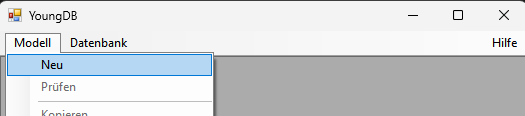
\includegraphics[width=0.4\textwidth]{img/YDB_ModellNeu.png}
    \item Lege \emphColB{zwei neue Klassen} an, bearbeite sie mit \emph{Doppelklick} und erstelle jeweils einen \emphColB{ganzzahligen Primärschlüssel id}.\\\\
    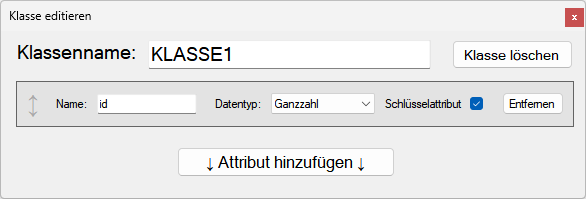
\includegraphics[width=0.5\textwidth]{img/YDB_idErstellen.png}
    \item Erstelle eine Beziehung zwischen den beiden Klassen, indem du mit \emph{Rechtsklick, Halten und Ziehen} eine rote Linie aus einer der Klassen zur anderen ziehst und dann die Maus loslässt. Bearbeite die Beziehung anschließend mit \emph{Doppelklick}, sodass sie eine \emphColB{1:n Beziehung von Klasse2 zu Klasse1} ist.\\\\
    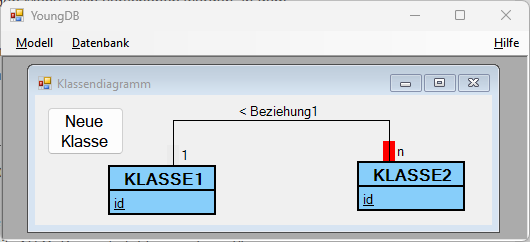
\includegraphics[width=0.5\textwidth]{img/YDB_1nBeziehung.png}\\
    \emph{Tipp:} Klassen kannst du per Doppelklick und \emph{Klasse löschen} entfernen und eine Beziehung, indem du den roten Kasten, der erscheint, wenn deine Maus am Anfang der Linie ist, irgendwo hin ziehst.
    \item \emphColB{Beantworte:} Welche Unterschiede stellst du zu normalen Klassendiagrammen fest?\\\LoesungLine{keine Datentypen, }{2}
    \item Erstelle aus dem Modell eine \emphColB{neue Datenbank und speichere sie} auf deinem Laufwerk H:/. Verwende einen ähnlichen Namen wie für das Modell.Hier kannst du Tabellen öffnen, Daten eintragen, SQL-Abfrage schreiben, speichern und laden.\\\\
    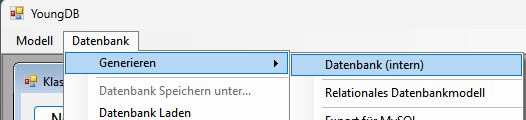
\includegraphics[width=0.45\textwidth]{img/YDB_dbGenerieren.png}
\end{enumerate}





        %\Aufgabe{m:n-Beziehungen}

\begin{enumerate}
    \item Erstelle in YoungDB ein Datenbankmodell mit den Klassen Lehrkraft und Schulklasse, die in einer m:n-Beziehung zueinander stehen. Überlege dir sinnvolle Primärschlüssel und 1-2 Attribute und eine sinnvolle Bezeichnung für die Beziehung.
    \item Generiere nun die zugehörige Datenbank und befülle die Tabellen mit jeweils 2-3 Datensätzen.
    \item Beantworte folgende Fragen:\begin{itemize}
        \item Welchen essentiellen Unterschied gibt es zwischen m:n-Beziehungen und 1:n-/1:1-Beziehungen?\\
        \LoesungLine{Beziehungstabelle benötigt}{1}
        \item Was für Datensätze werden in der dritten Tabelle eingetragen?\\
        \LoesungLine{Paare von IDs der Datensätze der anderen Tabellen, die in Beziehung zueinander stehen}{2}
        \item Welche Spalten welcher Tabelle(n) sind Fremdschlüssel?\\\LoesungLine{beide Spalten der dritten Beziehungstabelle}{1}
        \item Welche Spalte(n) sind Primärschlüssel in der dritten Tabelle? \emph{Tipp: Was muss eindeutig sein? Probiere deine Vermutung aus, indem du versucht mehrere Datensätze mit gleichem (vermuteten) Primärschlüssel einzufügen.} 
        \\\LoesungLine{beide Spalten zusammen}{1}
        \item Ist es sinnvoll bei m:n-Beziehungen im Klassendiagramm eine Richtung anzugeben und wieso?
        \\\LoesungLine{}{2}
        \item Wie könnte man m:n-Beziehung im Klassendiagramm alternativ darstellen?
        \\\LoesungLine{zusätzliche Beziehungstabelle mit zwei 1:n-Beziehungen}{1}
        \item Zeichne die Darstellung von m:n-Beziehungen in YoungDB ein:\\\\
        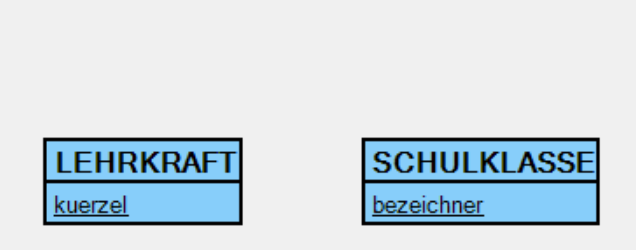
\includegraphics[width=0.6\textwidth]{Aufgaben/img/YDB_lehrerKlasse.png}
    \end{itemize}
\end{enumerate} 

        %\Hefteintrag{1.9}{Darstellung von m:n-Beziehungen}{

m:n-Beziehungen können im UML-Klassendiagramm auf zwei verschiedene Arten dargestellt werden:
\vspace{0.5cm}

\emphOrange{1. \LoesungLuecke{als direkte Beziehung}{15cm}}\\
Vorteil: \LoesungLuecke{Diagramm kompakt und übersichtlich}{15cm}

\vspace{0.5cm}
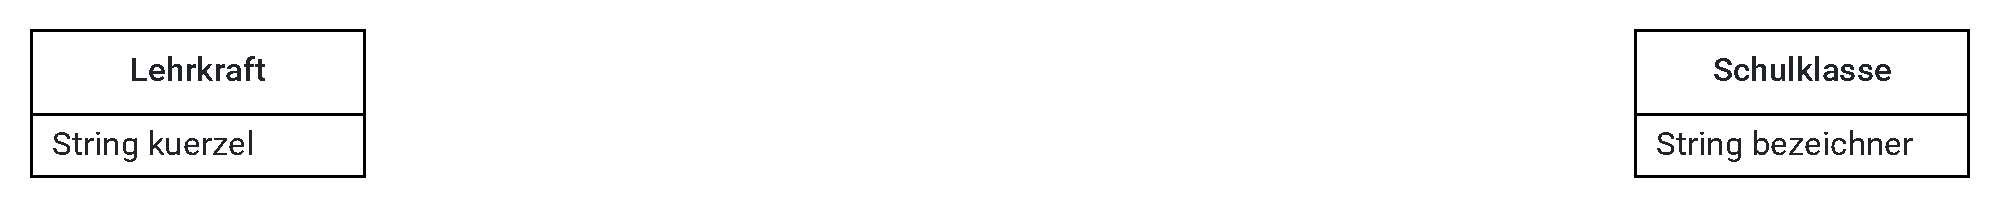
\includegraphics[width=\textwidth]{Aufgaben/img/mn-Beispiel}


\emphOrange{2. \LoesungLuecke{mit Beziehungstabelle}{15cm}}\\
Vorteil: \LoesungLuecke{Diagramm kompakt und übersichtlich}{15cm}

\vspace{1.5cm}
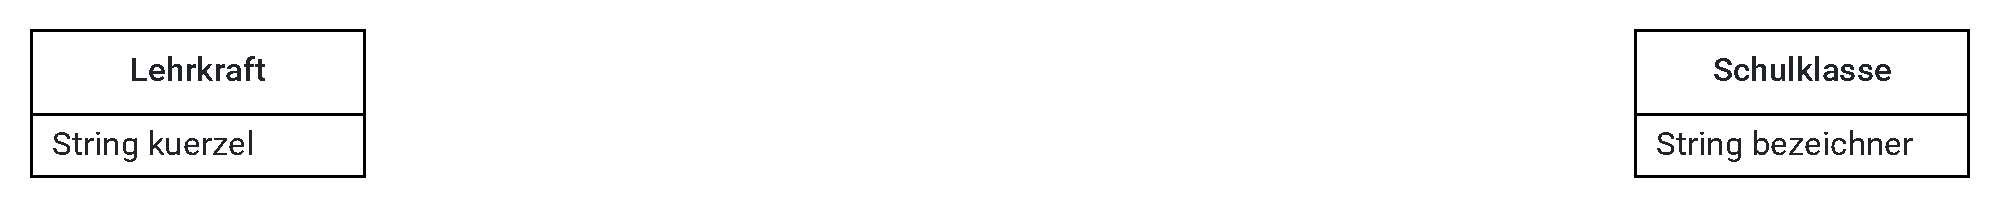
\includegraphics[width=\textwidth]{Aufgaben/img/mn-Beispiel}\\

}

        %\Hefteintrag{1.9}{SQL-Abfragen mit Join bei m:n-Beziehungen}{
Um zwei Tabellen, die eine m:n-Beziehung miteinander haben, zu joinen (also ihren Join zu bilden und in der Ergebnistabelle nur \LoesungLuecke{zusammengehörende}{7cm} Datensätze zu haben), muss man:
\begin{itemize}
    \item Daten aus allen \LoesungLuecke{drei}{2cm} Tabellen abfragen (also diese nach \emphOrange{\LoesungLuecke{FROM}{3cm}} auflisten).
    \item Die \emphOrange{\LoesungLuecke{Beziehungstabelle}{8cm}} einzeln mit den normalen Tabellen joinen. Hierfür benötigt man \emphOrange{\LoesungLuecke{zwei}{2cm}} Join-Bedingungen, die mit \emphOrange{\LoesungLuecke{AND}{2cm}} verknüpft werden.
\end{itemize}

\emphOrange{Beispiel:}

\emphGreen{SELECT} Lehrkraft.*, Schulklasse.*\\
\emphGreen{FROM} Lehrkraft, Schulklasse, \emphBlue{\LoesungLuecke{Lehrer\_unterricht\_Klasse}{10cm}}\\
\emphGreen{WHERE} \emphBlue{Lehrer\_unterricht\_Klasse.lehrer} = \LoesungLuecke{Lehrkraft.kuerzel}{8cm} \\
\emphGreen{AND}  \emphBlue{Lehrer\_unterricht\_Klasse.klasse} = \LoesungLuecke{Schulklasse.bezeichner}{8cm}

}


        %\begin{minipage}[t]{\textwidth}
\Aufgabe{Song-Datenbank Diagramme: \url{www.dbiu.de/songs}}

Zeichne die \emphColB{Klassenkarten} der Tabellen und \emphColB{Song und Playlist}. Zeichne anschließend mit \emphColC{zwei verschiedenen Farben} die beiden \emphColC{Darstellungsmöglichkeiten der Beziehung} zwischen den beiden Tabellen ein.

\LoesungKaro{\includegraphics[width=0.5\textwidth]{img/07_Songs.png}}{13}\\
    
\end{minipage}

        %%\Aufgabe{Song-Datenbank SQL}

Bearbeite dann folgende SQL-Aufgaben auf der Website \url{www.dbiu.de/songs} und notiere die getesteten Abfragen. 


\begin{enumerate}
    
    %\item  Welche Songs (alle Attribute) gibt es insgesamt?\\
    %\LoesungLine{SELECT * FROM Song}{1}
    
    %\item Welche IDs haben die Songs, die in irgendeiner Playlist enthalten sind?\\
    %\LoesungLine{SELECT Song.id FROM Song, Song\_in\_Playlist WHERE Song\_in\_Playlist.song\_id = Song.id}{2}
    
    \item Welche Songs (alle Attribute) sind in irgendeiner Playlist enthalten?\\
    \LoesungLine{SELECT Song.* 
    FROM Song, Song\_in\_Playlist 
    WHERE Song\_in\_Playlist.song\_id = Song.id}{2}
    
    \item Gib die Titel aller Playlists und die Titel der jeweils zugehörigen Songs aus.\\
    \LoesungLine{SELECT Playlist.titel, Song.titel
    FROM Song, Playlist, Playlist, Song\_in\_Playlist 
    WHERE Song\_in\_Playlist.song\_id = Song.id 
    AND Song\_in\_Playlist.playlist\_id = Playlist.id}{4}

    \item Welche Songs (alle Attribute) sind in der Playlist namens 'Fussballhits' enthalten?\\
    \LoesungLine{SELECT Song.* 
    FROM Song, Song\_in\_Playlist, Playlist 
    WHERE Song\_in\_Playlist.song\_id = Song.id 
    AND Song\_in\_Playlist.playlist\_id = Playlist.id
    AND Playlist.tiel = 'Fussballhits'}{5}
\end{enumerate}
    
}